\documentclass[compress, aspectratio=54]{beamer}
%\documentclass[notes=show]{beamer}
%\documentclass[xcolor=dvipsnames]{beamer}
\usepackage[export]{adjustbox}
\usepackage{sidecap}
\usepackage{subfig}
\usepackage{amssymb}
\usepackage{latexsym}
\usepackage{amsfonts}
\usepackage{amsmath}
\usepackage[absolute,overlay]{textpos}
\usepackage[english]{babel}
\usepackage[latin1]{inputenc}
\usepackage{subfig}
\usepackage{pythontex} 
\usepackage{listings}

%\usepackage{times}
\usepackage[T1]{fontenc}
\usepackage{tabularx}
\newcolumntype{Y}{>{\small\raggedright\arraybackslash}X}
\usepackage{graphicx}
\usepackage{bigstrut}
\usepackage{bbm}
\usepackage{mathrsfs}
\usepackage{epsfig}
\usepackage{array}
%\usepackage{natbib}
\usepackage{hyperref}
\usepackage{caption}
\usepackage{comment}

\mode<presentation> {
%\usetheme[left,width=1.7cm]{Berkeley}
%\usetheme{default}
\usetheme{Boadilla}
  \usecolortheme[RGB={103,102,204}]{structure}
%\usecolortheme{dove}
  \useoutertheme{infolines}
  \setbeamercovered{transparent}
 }

%\usepackage[utf8]{inputenc}

% Default fixed font does not support bold face
\DeclareFixedFont{\ttb}{T1}{txtt}{bx}{n}{12} % for bold
\DeclareFixedFont{\ttm}{T1}{txtt}{m}{n}{12}  % for normal

% Custom colors
\usepackage{color}
\definecolor{deepblue}{rgb}{0,0,0.5}
\definecolor{deepred}{rgb}{0.6,0,0}
\definecolor{deepgreen}{rgb}{0,0.5,0}

\usepackage{listings}

% Python style for highlighting
\newcommand\pythonstyle{\lstset{
language=Python,
basicstyle=\ttm,
otherkeywords={self},             % Add keywords here
keywordstyle=\ttb\color{deepblue},
emph={MyClass,__init__},          % Custom highlighting
emphstyle=\ttb\color{deepred},    % Custom highlighting style
stringstyle=\color{deepgreen},
frame=tb,                         % Any extra options here
showstringspaces=false            % 
}}


% Python environment
\lstnewenvironment{python}[1][]
{
\pythonstyle
\lstset{#1}
}
{}

% Python for external files
\newcommand\pythonexternal[2][]{{
\pythonstyle
\lstinputlisting[#1]{#2}}}

% Python for inline
\newcommand\pythoninline[1]{{\pythonstyle\lstinline!#1!}}
%\renewcommand{\familydefault}{cmss}
%\renewcommand{\mathrm}{\mathsf}
%\renewcommand{\textrm}{\textsf}
\usefonttheme{serif}
\newcommand{\X}{{\mathbf{X}}}
\newcommand{\x}{{\mathbf{x}}}
\newcommand{\E}{\mathsf{E}}
\newcommand{\V}{\mathsf{Var}}

\DeclareGraphicsExtensions{.jpg,.pdf,.mps,.png}

\setbeamercolor{bibliography entry title}{fg=black}
\setbeamercolor{bibliography entry author}{fg=black}
\setbeamercolor{subsection in toc}{fg=structure}
\setbeamercolor{palette primary}{bg=structure, fg=white}
%\setbeamercolor{palette secondary}{bg=structure, fg=black}
%\setbeamercolor{palette tertiary}{bg=structure, fg=black}
\setbeamercolor{caption name}{fg=black} \setbeamersize{text margin
left=.8cm} \setbeamersize{text margin right=1cm}
\hypersetup{linkbordercolor={1 0 0}} \setbeamertemplate{navigation
symbols}{} \setbeamertemplate{headline}[default]

\setbeamertemplate{enumerate items}[default]

\newcounter{transfct}
\newcounter{begbs}
\newcounter{endbs}


\title[Word Embeddings]{Machine Learning for Natural Language Processing}

\author[Arieda Mu\c co]{Arieda Mu\c co}
\institute[CEU]{Central European University}

\AtBeginSection[] {
  \begin{frame}<handout:0>
    \frametitle{TOC}
    \tableofcontents[currentsection]
  \end{frame}
}

\date{}

\pgfdeclareimage[height=.7cm]{logo}{rgs2}
\logo{\pgfuseimage{logo}}
\begin{document}
\captionsetup[subfigure]{labelformat=empty}

\frame{\titlepage}

%%%%%%%%%%%%%%%%%%%%%%%%%%%%%%%%%%%%%%%%%%%


\begin{frame}
\frametitle{Word Embeddings}
\begin{itemize}
\item Fancy word, old concept
\item Vector representation of a word (we have already seen count-vectorizer, tf-idf) 
\item What we mean by word embedding is that we are embedding a categorical entity into a vector spacee
\end{itemize}
\end{frame}
%----------------------------------------------------------------------------%


%----------------------------------------------------------------------------%
\begin{frame}
\frametitle{Word Embeddings}
\begin{center}
    
\includegraphics[width=0.8\textwidth]{Figures/word-embeddings}
\end{center}
\end{frame}
%----------------------------------------------------------------------------%





\begin{frame}
\frametitle{Word Analogies}
\begin{figure}
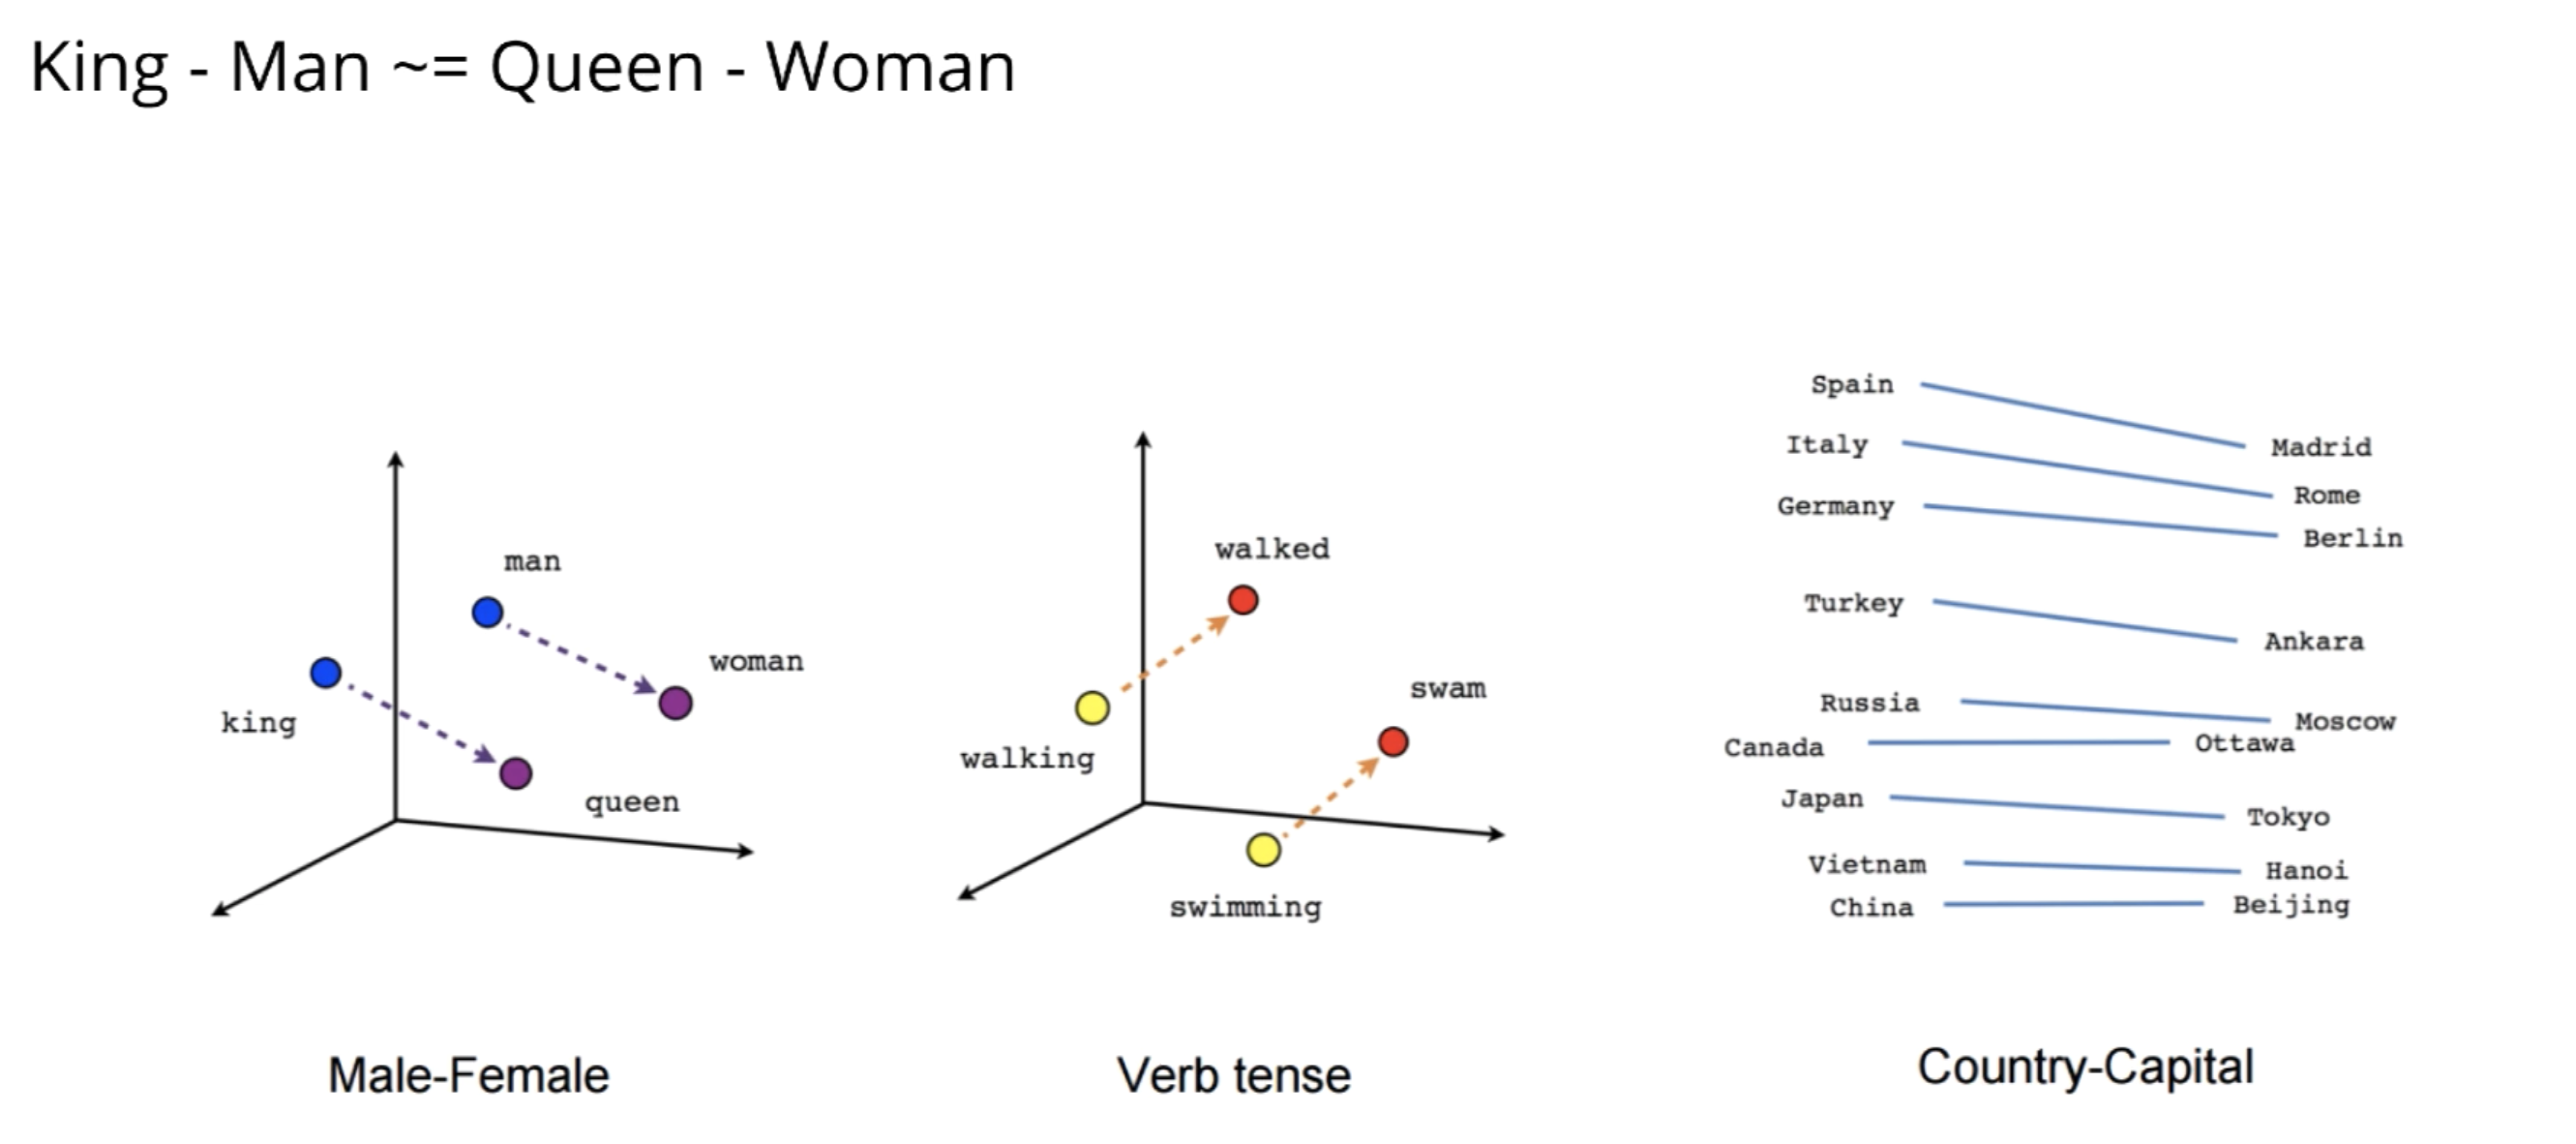
\includegraphics[width=1.1\linewidth ]{Figures/word-analogies}
\end{figure}

\end{frame}

%----------------------------------------------------------------------------%
\begin{frame}
\frametitle{Examples}
\begin{itemize}
\item King - Queen $\sim =$ Prince - Princess
\item France - Paris $\sim =$  Germany - Berlin
\item Japan - Japanese $\sim =$  China - Chinese
\item Brother - Sister $\sim = $ Uncle - Aunt
\item Walk - Walking $\sim =$  Swim - Swiming
\end{itemize}

\end{frame}

%----------------------------------------------------------------------------%
\begin{frame}
\frametitle{Visualizing Analogies}

\begin{center}
    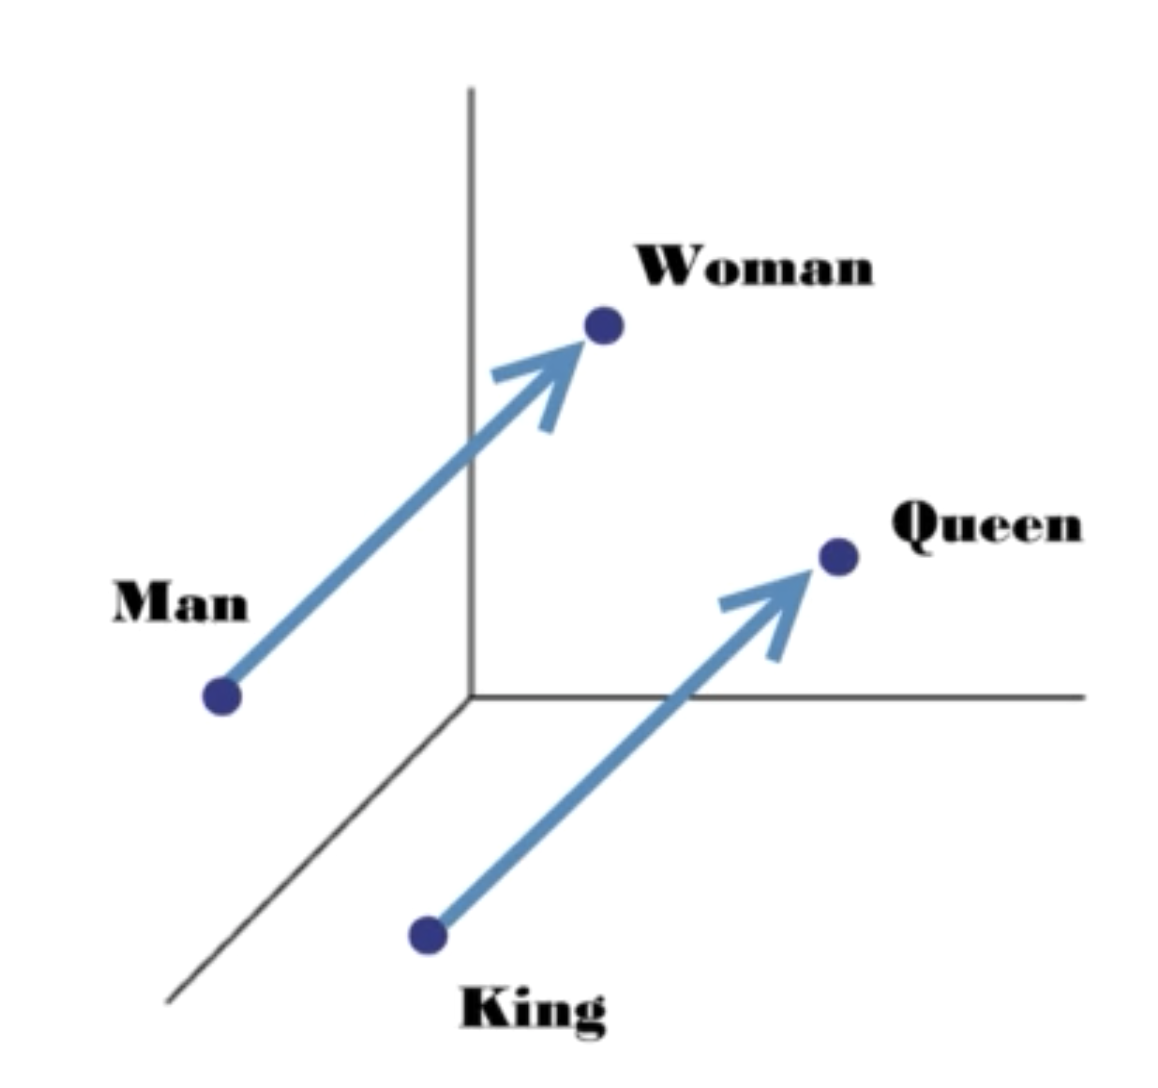
\includegraphics[width=0.7\textwidth]{Figures/visualizing-analogies}
\end{center}
\end{frame}
%----------------------------------------------------------------------------%
\begin{frame}
\frametitle{Code}

closest\_distance = infinity\\
best\_word = None\\
test\_vector = king - man + woman\\
for word, vector in vocabulary:\\
\hspace{10 mm}distance = get\_distance(test\_vector, vector):\\
\hspace{10 mm}if distance < closest\_distance:\\
\hspace{20 mm}closest\_distance = distance\\
\hspace{20 mm}best\_word = word\\
\vspace{10 mm}
\begin{itemize}
\item Use Numpy to do this
\item Use Cosine Distance  (or 1- Cosine Similarity) as a distance measure. Alternatively, use Euclidian Distance
\end{itemize}

\end{frame}


\end{document}

